% Beamer slide deck for Mathematical Physics
% "Mathematical Physics"
% Chapter 3: Method of Frobenius
% Self-contained: no external figures or bibliography.

\documentclass[11pt]{beamer}

\usepackage[utf8]{inputenc}
\usepackage[T1]{fontenc}
\usepackage{lmodern}
\usepackage{amsmath,amssymb}
\usepackage{graphicx}
\usepackage{tikz}

\usetheme{Madrid}

\author[]{Compiled by Jake W. Liu}
\title[Method of Frobenius]{Chapter 3: Method of Frobenius}
\subtitle{Mathematical Physics}
\date{\today}

\setbeamertemplate{navigation symbols}{}
\setbeamertemplate{frametitle continuation}[from second]

% Per-section TOC frames removed to keep the deck within 60 slides.

\usepackage{Kyushu}

% Neutralize \index so source markup (if any) is harmless.
\makeatletter
\@ifundefined{index}{\newcommand{\index}[1]{}}{\renewcommand{\index}[1]{}}
\makeatother

\begin{document}

\newcounter{sfchapter}
\setcounter{sfchapter}{3}
\renewcommand{\thesection}{\arabic{sfchapter}.\arabic{section}}
\numberwithin{equation}{section}

\begin{frame}[c]\titlepage
\end{frame}

\begin{frame}{Outline}
\tableofcontents
\end{frame}

\begin{frame}{Where we are going}
\footnotesize
Separation of variables turns many partial differential equations (PDEs) into linear,
second-order, homogeneous ordinary differential equations. Two recurring examples are
\begin{itemize}
  \item the \textbf{guitar string}, which gives the harmonic-oscillator equation
        \[
          \frac{d^2 y}{dx^2}+k^2y=0,
        \]
  \item the \textbf{drum}, which gives Bessel's equation
        \[
          x^2\frac{d^2y}{dx^2}+x\frac{dy}{dx}+(k^2x^2-m^2)y=0.
        \]
\end{itemize}
Here $k$ is a wave number, and $m$ is the nonnegative integer angular order of a drum
mode.
The string equation is solved by $\cos kx$ and $\sin kx$, but Bessel's equation has
no elementary solutions for integer $m$: we need a systematic series method.
On an interval where the coefficient of $y''$ is nonzero, a linear homogeneous
second-order equation can be written as
\[
  y''+P(x)y'+Q(x)y=0.
\]
Here \emph{linear} means that $y,y',y''$ occur only to the first power and are not
multiplied together; \emph{homogeneous} means that the right-hand side is zero.  The
method of Frobenius is such a series method for this class of equations; it succeeds
at ordinary points and regular singular points, defined later.
\end{frame}

% ======================================================================
\section{The guitar string and the drum head}
% ======================================================================

\begin{frame}[allowframebreaks=1.00]{Guitar string: the harmonic oscillator by Taylor series}
\footnotesize

\textbf{Goal.} Find every solution of the string equation below, and the wave numbers $k$ for
which it can vanish at both ends. We know the answer ($\cos$ and $\sin$) from calculus; the point
is to find it with a power-series method that will also work for Bessel's equation.

\textbf{Step 1: insert a power series.}  A string of length $L$ fixed at both ends obeys
\[
 \frac{d^2y}{ds^2}+k^2y=0,\qquad 0\le s\le L,\qquad y(0)=y(L)=0.
\]
First remove \(k\) by a change of variable: \(x=ks\). By the chain rule, \(\frac{dy}{ds}=k\frac{dy}{dx}\) and
\(\frac{d^2y}{ds^2}=k^2\frac{d^2y}{dx^2}\). So the equation reads \(k^2y''+k^2y=0\); dividing by \(k^2\),
\begin{equation}
  y''+y=0,
  \label{eq:ho}
\end{equation}
and the ends move to \(x=0\) and \(x=kL\). We solve \eqref{eq:ho} first and impose the end
conditions afterwards.

\textbf{The idea.} Guess that the solution is a ``polynomial of infinite degree'' (a power series)
with unknown coefficients. Substituting it into the equation gives conditions that fix the
coefficients one after another. Write
\[
  y(x)=\sum_{n=0}^{\infty}a_nx^n
      =a_0+a_1x+a_2x^2+a_3x^3+\cdots.
\]
Term-by-term differentiation gives
\[
\begin{aligned}
  y'(x)
    &=\sum_{n=1}^{\infty}n a_nx^{n-1}
      =a_1+2a_2x+3a_3x^2+\cdots,\\
  y''(x)
    &=\sum_{n=2}^{\infty}n(n-1)a_nx^{n-2}
      =2a_2+3\cdot2a_3x+4\cdot3a_4x^2+\cdots.
\end{aligned}
\]
Substitution into \eqref{eq:ho} yields
\[
  \sum_{n=2}^{\infty}n(n-1)a_nx^{n-2}
  +\sum_{n=0}^{\infty}a_nx^n=0.
\]
\textbf{Step 2: align the powers.}  The powers do not yet match.  Reindexing aligns every
sum on the same power of $x$.  In the first sum set
\[
  j=n-2,
  \qquad n=j+2.
\]
When $n=2$, $j=0$, and as $n\to\infty$, $j\to\infty$.  Therefore
\[
\begin{aligned}
  \sum_{n=2}^{\infty}n(n-1)a_nx^{n-2}
    &=\sum_{j=0}^{\infty}(j+2)(j+1)a_{j+2}x^j\\
    &=\sum_{n=0}^{\infty}(n+2)(n+1)a_{n+2}x^n,
\end{aligned}
\]
where the last line only renames the dummy index $j$ as $n$.  Hence
\[
  \sum_{n=0}^{\infty}
  \left[(n+2)(n+1)a_{n+2}+a_n\right]x^n=0.
\]
\textbf{Step 3: read off the recurrence.}  A power series is identically zero only when each coefficient is zero.  Thus, for every
$n\ge0$,
\[
  (n+2)(n+1)a_{n+2}+a_n=0,
\]
and solving for the next coefficient gives
\begin{equation}
  a_{n+2}=-\frac{a_n}{(n+1)(n+2)},
  \qquad n=0,1,2,\ldots.
  \label{eq:ho-rec}
\end{equation}
The recurrence advances the index by two.  Consequently, $a_0$ generates all even
coefficients, while $a_1$ generates all odd coefficients.
\end{frame}

\begin{frame}{Resolving the even recurrence into $\cos x$}
\footnotesize
Starting with $a_0$, the recurrence \eqref{eq:ho-rec} gives
\[
 a_2=-\frac{a_0}{1\cdot2}=-\frac{a_0}{2!},\qquad
 a_4=-\frac{a_2}{3\cdot4}=\frac{a_0}{4!}.
\]
Each step introduces the next two factors and reverses the sign, so after $j$ steps the
denominator is $(1\cdot2)(3\cdot4)\cdots\bigl((2j-1)(2j)\bigr)=(2j)!$. Hence
\[
 a_{2j}=\frac{(-1)^j a_0}{(2j)!},\qquad j=0,1,2,\ldots.
\]
The even part of the solution is therefore
\[
 a_0\left(1-\frac{x^2}{2!}+\frac{x^4}{4!}-\cdots\right)=a_0\cos x.
\]
This is the cosine Taylor series from Chapter~1, now recovered from the differential equation.
\end{frame}

\begin{frame}{Resolving the odd recurrence into $\sin x$}
\footnotesize
Starting with $a_1$ instead, the recurrence \eqref{eq:ho-rec} with $n=1$ and then $n=3$ gives
\[
 a_3=-\frac{a_1}{2\cdot3}=-\frac{a_1}{3!},\qquad
 a_5=-\frac{a_3}{4\cdot5}=\frac{a_1}{5!}.
\]
Each step again reverses the sign and contributes the next two factors, so after $j$ steps the sign is $(-1)^j$ and the denominator is $(2\cdot3)(4\cdot5)\cdots\bigl((2j)(2j+1)\bigr)=(2j+1)!$. Hence
\[
 a_{2j+1}=\frac{(-1)^j a_1}{(2j+1)!},\qquad j=0,1,2,\ldots,
\]
so the odd part is $a_1(x-x^3/3!+x^5/5!-\cdots)=a_1\sin x$.
Both starting coefficients are free, giving
\[
 y(x)=a_0\cos x+a_1\sin x,\qquad a_0=y(0),\quad a_1=y'(0).
\]
The differential equation determines the shape; endpoint or initial conditions determine
which combination is needed.
\end{frame}

\begin{frame}{Applying the endpoint conditions}
\footnotesize
The string is fixed at its left end, so $y(0)=a_0=0$.
The right end $s=L$ is $x=kL$. Thus
\[
 0=y(kL)=a_1\sin(kL).
\]
A nonzero mode has $a_1\ne0$, so
\[
 kL=n\pi,\qquad\text{i.e.}\qquad k_n=\frac{n\pi}{L},\qquad n=1,2,\ldots.
\]
The $n$th mode is $y=A\sin x=A\sin(k_ns)$; the fundamental $n=1$ is half a sine wave
along the string.  The frequency of a mode is proportional to its wave number, so all
frequencies are integer multiples of the lowest one: this is why a string sounds
\emph{harmonic}.  The drum will turn out differently.

The end conditions do not determine the amplitude $A$; an additional
amplitude or normalization condition is needed.
\end{frame}

\begin{frame}[allowframebreaks=1.00]{Drum: Bessel's equation needs a generalized series}
\footnotesize

\textbf{Goal.} Solve the radial equation of a vibrating circular drum by a series, as we did for
the string. We will see that a plain Taylor series is not enough, and why.

\textbf{Step 1: the equation, in scaled form.} For a circular drum, separating the angle gives
the radial equation below (the separation itself is done at the start of Chapter~5):
\[
 \rho^2Y''(\rho)+\rho Y'(\rho)+(k^2\rho^2-m^2)Y(\rho)=0.
\]
Here \(\rho\) is the distance from the center, \(k>0\) is a wave number, and the integer \(m\ge0\) counts
how the mode varies around the drum. Remove \(k\) by putting \(x=k\rho\), \(Y(\rho)=y(x)\). By the
chain rule \(Y'(\rho)=k\,y'(x)\) and \(Y''(\rho)=k^2y''(x)\). Term by term, using \(k\rho=x\):
\[
 \rho^2Y''=(k\rho)^2y''=x^2y'',\qquad \rho Y'=(k\rho)\,y'=xy',\qquad (k^2\rho^2-m^2)Y=(x^2-m^2)y .
\]
This gives Bessel's equation
\begin{equation}
 x^2y''+xy'+(x^2-m^2)y=0.\label{eq:bessel}
\end{equation}
The rim \(\rho=R\) is now \(x=kR\); we return to it once we have a solution.
\par\framebreak\par
\textbf{Step 2: why a plain Taylor series is not enough.} Divide \eqref{eq:bessel} by \(x^2\):
\[
 y''+\frac1x\,y'+\Bigl(1-\frac{m^2}{x^2}\Bigr)y=0 .
\]
The coefficients \(1/x\) and \(m^2/x^2\) blow up at \(x=0\). Such a point is called a \emph{singular point}.
Near it, solutions can behave like \(x^{-m}\) or \(\log x\), which no Taylor series can represent.

\textbf{Step 3: guess how solutions start.} Suppose \(y\approx x^r\) near \(x=0\), for some power \(r\) to be
found. Compare the sizes of the four terms of \eqref{eq:bessel}:
\[
 x^2y''\sim x^r,\qquad xy'\sim x^r,\qquad m^2y\sim x^r,\qquad x^2y\sim x^{r+2}.
\]
Near \(x=0\) the last term is much smaller than the others. Dropping it leaves
\(x^2y''+xy'-m^2y=0\), an \emph{Euler equation}. Try \(y=x^r\): \(x^2\cdot r(r-1)x^{r-2}+x\cdot rx^{r-1}-m^2x^r
=\bigl[r(r-1)+r-m^2\bigr]x^r=(r^2-m^2)x^r\). So \(r=\pm m\).

\textbf{Conclusion.} Solutions should start like \(x^r\) (a power that need not be a whole number),
followed by higher powers that the dropped term \(x^2y\) brings in. So on \(x>0\) we try the
\emph{Frobenius ansatz}:
\begin{equation}
  y(x)=x^r\sum_{n=0}^{\infty}a_nx^n
      =\sum_{n=0}^{\infty}a_nx^{n+r},
  \qquad a_0\ne0.
  \label{eq:frob-series}
\end{equation}
Here \(r\) is unknown and will be determined. Differentiate term by term. Unlike the Taylor case,
every sum still starts at \(n=0\): since \(r\) is not a known whole number, the \(n=0\) term does not
drop out (and it is exactly the term that will determine \(r\)):
\[
\begin{aligned}
  y'(x)
    &=\sum_{n=0}^{\infty}(n+r)a_nx^{n+r-1},\\
  y''(x)
    &=\sum_{n=0}^{\infty}(n+r)(n+r-1)a_nx^{n+r-2}.
\end{aligned}
\]
\par\framebreak\par
\textbf{Step 4: substitute and align powers.}  Substitute into \eqref{eq:bessel}. Multiplying
\(x^2\) into \(x^{n+r-2}\), \(x\) into \(x^{n+r-1}\), and \(x^2-m^2\) into \(x^{n+r}\) gives
\[
\begin{aligned}
0={}&\sum_{n=0}^{\infty}(n+r)(n+r-1)a_nx^{n+r}
+\sum_{n=0}^{\infty}(n+r)a_nx^{n+r}\\
&+\sum_{n=0}^{\infty}a_nx^{n+r+2}
-m^2\sum_{n=0}^{\infty}a_nx^{n+r}.
\end{aligned}
\]
Only the third sum has the shifted power $x^{n+r+2}$.  Set $j=n+2$, so $n=j-2$:
\[
  \sum_{n=0}^{\infty}a_nx^{n+r+2}
    =\sum_{j=2}^{\infty}a_{j-2}x^{j+r}
    =\sum_{n=2}^{\infty}a_{n-2}x^{n+r}.
\]
With the bookkeeping convention $a_{-2}=a_{-1}=0$, this last sum may start at $n=0$
without adding nonzero terms.
\par\framebreak\par
\textbf{Step 5: collect and read off the conditions.}  All four sums now carry \(x^{n+r}\):
\[
  \sum_{n=0}^{\infty}
  \left[
    (n+r)(n+r-1)a_n+(n+r)a_n-m^2a_n+a_{n-2}
  \right]x^{n+r}=0.
\]
Since
\[
  (n+r)(n+r-1)+(n+r)
  =(n+r)\bigl[(n+r-1)+1\bigr]
  =(n+r)^2,
\]
and a power series is zero only if every coefficient is zero, the coefficient equation is
\begin{equation}
  \left[(n+r)^2-m^2\right]a_n+a_{n-2}=0,
  \qquad n=0,1,2,\ldots.
  \label{eq:bessel-coeff}
\end{equation}
\textbf{The lowest power, \(n=0\),} fixes \(r\). There \(a_{-2}=0\), so \((r^2-m^2)a_0=0\). Because \(a_0\ne0\) (by
assumption, \(x^r\) is the true starting power), we get the \emph{indicial equation}
\begin{equation}
  r^2-m^2=0
  \quad\Longleftrightarrow\quad
  (r-m)(r+m)=0,
  \label{eq:indicial-bessel}
\end{equation}
so $r=m$ or $r=-m$, the exponents the Euler equation predicted.
Near $x=0$ the solution behaves like $a_0x^r$.  For $m\ge1$, the root $r=-m$ gives
$x^{-m}$, which blows up at the drum's center, while $r=m\ge0$ gives a solution that
stays finite there (for $m=0$ the two roots coincide).
\end{frame}

\begin{frame}[allowframebreaks=1.00]{The Bessel recurrence and $J_m(x)$}
\footnotesize
\textbf{Goal.} Use the regular root \(r=m\) to compute all the coefficients \(a_n\), and so obtain the
solution that is finite at the drum's center.

\textbf{Step 1: simplify the coefficient equation.} With \(r=m\),
\((n+m)^2-m^2=n^2+2nm=n(n+2m)\), so \eqref{eq:bessel-coeff} becomes
\begin{equation}
 n(n+2m)\,a_n+a_{n-2}=0,\qquad\text{that is,}\qquad a_n=-\frac{a_{n-2}}{n(n+2m)}\quad(n\ge1).
 \label{eq:bessel-rec}
\end{equation}
Each coefficient is fixed by the one two steps back.

\textbf{Step 2: the odd coefficients vanish.} At \(n=1\): \(1\cdot(1+2m)\,a_1+a_{-1}=0\), and \(a_{-1}=0\), so
\(a_1=0\). Then \(a_3=-a_1/(3(3+2m))=0\), \(a_5=0\), and so on: all odd coefficients are zero.

\textbf{Step 3: the first even coefficients.} Take \(n=2\), then \(n=4\):
\[
\begin{aligned}
 a_2&=-\frac{a_0}{2(2+2m)}=-\frac{a_0}{4(m+1)},\\
 a_4&=-\frac{a_2}{4(4+2m)}=-\frac{a_2}{8(m+2)}
     =-\frac{1}{8(m+2)}\cdot\Bigl(-\frac{a_0}{4(m+1)}\Bigr)=\frac{a_0}{32(m+1)(m+2)}.
\end{aligned}
\]
\par\framebreak\par
\textbf{Step 4: the general even coefficient.} At \(n=2j\) the factor in \eqref{eq:bessel-rec} is
\(2j(2j+2m)=4j(j+m)\). So each step multiplies by \(-1/[4j(j+m)]\). After \(j\) steps,
\[
 a_{2j}=a_0\cdot\frac{-1}{4\cdot1\cdot(1+m)}\cdot\frac{-1}{4\cdot2\cdot(2+m)}\cdots\frac{-1}{4\cdot j\cdot(j+m)} .
\]
Collect the pieces: \(j\) signs give \((-1)^j\), \(j\) fours give \(4^j\), the numbers \(1,2,\dots,j\) give \(j!\):
\[
 a_{2j}=\frac{(-1)^j\,a_0}{4^{j}\;j!\;(m+1)(m+2)\cdots(m+j)} .
\]
\textbf{Step 5: tidy with factorials.} Use \((m+1)(m+2)\cdots(m+j)=\frac{(m+j)!}{m!}\) and \(4^j=2^{2j}\):
\begin{equation}
 a_{2j}=\frac{(-1)^j\,m!\,a_0}{2^{2j}\,j!\,(m+j)!},\qquad a_{2j+1}=0.
 \label{eq:bessel-coeffs}
\end{equation}
\textbf{Step 6: choose the scale.} The equation is linear, so \(a_0\) is free. The standard choice
\(a_0=1/(2^m\,m!)\) cancels the \(m!\). Then each term of \eqref{eq:frob-series} with \(r=m\) is
\[
 a_{2j}x^{2j+m}=\frac{(-1)^j}{j!\,(m+j)!}\cdot\frac{x^{2j+m}}{2^{2j+m}}
 =\frac{(-1)^j}{j!\,(m+j)!}\left(\frac{x}{2}\right)^{2j+m}.
\]
Summing gives the \emph{Bessel function of the first kind}:
\begin{equation}
 J_m(x)=\sum_{j=0}^{\infty}\frac{(-1)^j}{j!\,(m+j)!}
           \left(\frac{x}{2}\right)^{2j+m},\qquad m=0,1,2,\ldots.
 \label{eq:Jm}
\end{equation}
For example, \(J_0(x)=1-\frac{x^2}{4}+\frac{x^4}{64}-\cdots\).
\end{frame}

\begin{frame}[allowframebreaks=1.00]{What the other Bessel root is trying to say}
\footnotesize

\textbf{The question.} A second-order equation has two independent solutions. The root \(r=+m\)
gave one (finite at the center). What does the other root \(r=-m\) give?

To include noninteger orders later, write the order as \(\nu\) (so the equation has \(\nu^2\) in place of
\(m^2\)). Put \(r=-\nu\) in \eqref{eq:bessel-coeff}. Since \((n-\nu)^2-\nu^2=n^2-2n\nu=n(n-2\nu)\),
\begin{equation}
 n(n-2\nu)\,a_n+a_{n-2}=0.
 \label{eq:bessel-negative-root-rec}
\end{equation}
\textbf{Integer order: the pure series fails.} Before dividing by \(n(n-2\nu)\), check whether it can
be zero. Take the drum mode \(\nu=m=1\): the equation is \(n(n-2)a_n+a_{n-2}=0\).
\begin{itemize}
  \item At \(n=2\) it reads \(0\cdot a_2+a_0=0\), so \(a_0=0\). But we assumed \(a_0\ne0\). Contradiction.
  \item For any integer \(m\ge1\) the same happens at \(n=2m\): the factor \(n(n-2m)\) is zero there, but
        \(a_{2m-2}\) (a nonzero multiple of \(a_0\)) is not.
  \item For \(m=0\) the two roots are the same, \(r=0\), so there is only one series anyway.
\end{itemize}
So for integer order the second solution is not a pure Frobenius series. It is called \(Y_m\); it
blows up at the origin, and we construct it later in this chapter by reduction of order.
\par\framebreak\par
\textbf{Noninteger order: both roots work.} Now let \(\nu>0\) not be an integer.

\emph{The root \(r=+\nu\).} Repeat Steps~1--5 of the previous frame with \(\nu\) in place of \(m\):
\[
 a_{2j}=\frac{(-1)^j\,a_0}{2^{2j}\,j!\,(\nu+1)(\nu+2)\cdots(\nu+j)} .
\]
The product \((\nu+1)\cdots(\nu+j)\) is no longer a ratio of factorials, but it is a ratio of gamma
functions. Apply \(\Gamma(z+1)=z\Gamma(z)\) (Chapter~2) \(j\) times:
\[
 \Gamma(\nu+j+1)=(\nu+j)\,\Gamma(\nu+j)=\cdots=(\nu+j)(\nu+j-1)\cdots(\nu+1)\,\Gamma(\nu+1),
\]
so \((\nu+1)\cdots(\nu+j)=\Gamma(\nu+j+1)/\Gamma(\nu+1)\). Choosing \(a_0=1/[2^\nu\Gamma(\nu+1)]\) (the analogue of
\(1/(2^mm!)\)), the \(\Gamma(\nu+1)\) cancels and
\[
 J_{\nu}(x)=\sum_{j=0}^{\infty}
 \frac{(-1)^j}{j!\,\Gamma(j+\nu+1)}\left(\frac{x}{2}\right)^{2j+\nu},
 \qquad x>0.
\]
\par\framebreak\par
\emph{The root \(r=-\nu\).} In \eqref{eq:bessel-negative-root-rec} the even-index factors are
\(2j(2j-2\nu)\), which are never zero because \(\nu\) is not an integer. So nothing goes wrong, and the
same calculation with \(\nu\) replaced by \(-\nu\) gives a second solution \(J_{-\nu}\).

\textbf{They are independent.} Look at the first terms (\(j=0\)) as \(x\to0^+\):
\[
 J_\nu(x)\approx\frac{(x/2)^\nu}{\Gamma(\nu+1)}\longrightarrow0,\qquad
 J_{-\nu}(x)\approx\frac{(x/2)^{-\nu}}{\Gamma(1-\nu)}\longrightarrow\infty .
\]
One tends to zero and the other blows up, so neither is a constant multiple of the other.
\par\framebreak\par
\textbf{Example: half order gives elementary functions.} Take \(\nu=\frac12\), so \(2\nu=1\), and
\eqref{eq:bessel-negative-root-rec} reads \(n(n-1)a_n+a_{n-2}=0\).
\begin{itemize}
  \item At \(n=0\) and \(n=1\) the factor \(n(n-1)\) is zero and \(a_{-2}=a_{-1}=0\): the equation is
        \(0=0\). So both \(a_0\) and \(a_1\) are free.
  \item For \(n\ge2\): \(a_n=-a_{n-2}/[n(n-1)]\). This is exactly the string recurrence \eqref{eq:ho-rec}
        (shifted by two). So \(\sum_na_nx^n=a_0\cos x+a_1\sin x\).
  \item Restore the factor \(x^r=x^{-1/2}\): \(\;y(x)=x^{-1/2}\bigl(a_0\cos x+a_1\sin x\bigr)\).
\end{itemize}
\textbf{Which combination is \(J_{\pm1/2}\)?} \(J_{-1/2}\) contains only the powers
\(x^{2j-1/2}=x^{-1/2}x^{2j}\) (even powers after \(x^{-1/2}\)): it is the \(\cos\) part. \(J_{1/2}\) contains only
\(x^{2j+1/2}=x^{-1/2}x^{2j+1}\): it is the \(\sin\) part. Match the leading terms, using
\(\Gamma(\frac12)=\sqrt\pi\) and \(\Gamma(\frac32)=\sqrt\pi/2\):
\[
 J_{-1/2}\approx\frac{(x/2)^{-1/2}}{\Gamma(1/2)}=\sqrt{\frac2\pi}\,x^{-1/2},
 \qquad
 J_{1/2}\approx\frac{(x/2)^{1/2}}{\Gamma(3/2)}=\sqrt{\frac2\pi}\,x^{1/2}.
\]
Since \(x^{-1/2}\cos x\approx x^{-1/2}\) and \(x^{-1/2}\sin x\approx x^{1/2}\), we get \(a_0=a_1=\sqrt{2/\pi}\):
\[
 J_{-1/2}(x)=\sqrt{\frac{2}{\pi x}}\cos x,\qquad
 J_{1/2}(x)=\sqrt{\frac{2}{\pi x}}\sin x.
\]
So a ``special'' function can be elementary at particular orders.
\end{frame}

\begin{frame}{The Bessel functions of the first kind $J_0,\dots,J_3$}
\footnotesize
\begin{center}
  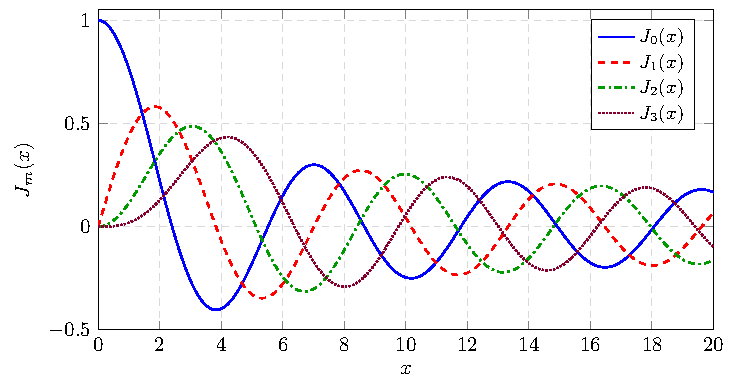
\includegraphics[width=0.86\linewidth]{figs/bessel-J.pdf}
\end{center}
Near the origin, $J_0(0)=1$, while $J_m(0)=0$ for every integer $m\ge1$: a drum mode that
varies with angle must vanish at the center.  The next frame gives the local and
large-$x$ formulas behind the picture.
\end{frame}

\begin{frame}[allowframebreaks=1.00]{Bessel asymptotics and drum eigenvalues}
\footnotesize
\textbf{Near the center (small \(x\)).} Take the first two terms of the series \eqref{eq:Jm}:
\[
 j=0:\ \frac{(x/2)^m}{m!},\qquad
 j=1:\ -\frac{(x/2)^{m+2}}{(m+1)!}=-\frac{(x/2)^m}{m!}\cdot\frac{(x/2)^2}{m+1}=-\frac{(x/2)^m}{m!}\cdot\frac{x^2}{4(m+1)},
\]
using \((m+1)!=(m+1)\,m!\). Factoring out the \(j=0\) term, for fixed \(m\),
\[
 J_m(x)=\frac1{m!}\left(\frac{x}{2}\right)^m
 \left[1-\frac{x^2}{4(m+1)}+O(x^4)\right]\qquad(x\to0).
\]
So \(J_0(0)=1\), while for \(m\ge1\), \(J_m\) vanishes at the center like \(x^m\).

\textbf{Far from the center (large \(x\)).} For fixed \(m\) and large positive \(x\) (Chapter~5 explains
where it comes from),
\[
  J_m(x)\approx\sqrt{\frac{2}{\pi x}}\;
  \cos\left(x-\frac{m\pi}{2}-\frac{\pi}{4}\right).
\]
So \(J_m\) oscillates like a cosine, with an amplitude that decays slowly, like \(x^{-1/2}\).
\par\framebreak\par
\textbf{The drum frequencies.} Let the drum have radius \(R\), clamped at the rim. The mode
\(J_m(k\rho)\) must vanish at \(\rho=R\): \(J_m(kR)=0\). Write \(\alpha_{m,n}\) for the \(n\)-th positive zero of
\(J_m\). Then \(kR\) must be one of these zeros:
\[
 k_{m,n}=\frac{\alpha_{m,n}}{R}.
\]
The frequencies are proportional to \(k\), hence to the zeros of \(J_m\).

\textbf{A drum is not harmonic.} For \(m=0\), \(\alpha_{0,n}\approx2.405,\ 5.520,\ 8.654\), in ratios
\(1:2.30:3.60\). For the string the ratios were \(1:2:3\) (from \(kL=n\pi\)), which is why a string sounds
musical. The drum's overtones are not whole-number multiples of the lowest frequency.
\end{frame}

\begin{frame}[allowframebreaks=1.00]{Choose the series by classifying the point}
\footnotesize
\textbf{The question.} For the string a Taylor series worked; for the drum we needed an extra power
\(x^r\). How can we tell in advance which kind of series to use at a point \(x_0\)?

\textbf{Recipe.} Put the equation in the form \(y''+P(x)y'+Q(x)y=0\) and write \(z=x-x_0\). (A function is
\emph{analytic} at \(x_0\) if it equals a convergent Taylor series there.)
\begin{itemize}
 \item \textbf{Ordinary point:} \(P\) and \(Q\) are analytic at \(x_0\). A plain Taylor series gives both
       solutions. \emph{Example:} Airy's equation \(y''-xy=0\) at \(x_0=0\): \(P=0\), \(Q=-x\).
 \item \textbf{Regular singular point:} \(P\) or \(Q\) blows up at \(x_0\), but only mildly: \(zP\) and \(z^2Q\) are
       analytic. Use a power \(z^r\) times a Taylor series (Frobenius).
       \emph{Example:} Bessel at \(x_0=0\): \(P=1/x\), \(Q=1-m^2/x^2\), so \(xP=1\) and \(x^2Q=x^2-m^2\) are fine.
 \item \textbf{Irregular singular point:} worse blow-up; Frobenius is not guaranteed to work.
       \emph{Example:} \(x^4y''+2x^3y'+y=0\) at \(0\): \(Q=1/x^4\), and \(x^2Q=1/x^2\) still blows up
       (treated later in this chapter).
\end{itemize}
\textbf{Why this test?} Near a regular singular point, the equation looks like an Euler equation
(as we saw for Bessel), and Euler equations are solved by powers \(z^r\). We use the test as a recipe
now; the next section explains it.
\end{frame}

\begin{frame}{The method of Frobenius: the recipe}
\footnotesize
To analyze a linear second-order equation near $x=x_0$, with $z=x-x_0$:
\begin{enumerate}
  \item Divide by the coefficient of $y''$ to get $y''+P(x)y'+Q(x)y=0$ ($x_0$ itself
        may be a zero of that coefficient).
  \item Classify $x_0$. At an ordinary point, use a Taylor series with free
        initial coefficients. At a regular singular point, use
        \[
          y(x)=\sum_{k=0}^{\infty}a_k z^{k+r},\qquad a_0\ne0.
        \]
  \item Differentiate, reindex so the powers match, and equate coefficients, as in the
        string and Bessel examples.
  \item For a Frobenius series, set the coefficient of the lowest power to zero.
        This gives the \emph{indicial equation} for $r$.
  \item For each root $r$, solve the recurrence from the remaining coefficients.  Where
        its denominator vanishes, do not divide: go back to the undivided equation, which
        may force a coefficient, leave one free, or be contradictory (as at $n=2m$ for
        Bessel's root $r=-m$).
  \item Substitute back and check the result against the equation and any initial or
        boundary conditions.
\end{enumerate}
\end{frame}

\begin{frame}[allowframebreaks=1.00]{Example: Airy's equation by series}
\footnotesize
Airy's equation
\begin{equation}
 y''-xy=0\label{eq:airy}
\end{equation}
is the simplest model of a \emph{turning point}, where a wave (or a quantum particle)
passes from a region where it can propagate into one where it cannot.  Written as
$y''+\kappa^2y=0$ with $\kappa^2=-x$, the squared local wave number changes sign at $x=0$:
solutions oscillate for $x<0$ and grow or decay for $x>0$.

\textbf{Goal.} Find all solutions of \eqref{eq:airy} as power series about \(x=0\).

\textbf{Step 1: which series?} At \(x=0\), \(P=0\) and \(Q=-x\) are analytic, so \(x=0\) is an ordinary
point and a plain Taylor series is enough. Write
\[
 y=\sum_{n=0}^{\infty}a_nx^n,\qquad
 y'=\sum_{n=1}^{\infty}na_nx^{n-1}.
\]
Differentiate once more, then shift the index so that the power is $x^n$:
\[
 y''=\sum_{j=2}^{\infty}j(j-1)a_jx^{j-2}
     =\sum_{n=0}^{\infty}(n+2)(n+1)a_{n+2}x^n.
\]
For the other term, multiplication by $x$ shifts the coefficients in the opposite way:
\[
 xy=\sum_{j=0}^{\infty}a_jx^{j+1}
    =\sum_{n=1}^{\infty}a_{n-1}x^n.
\]
\par\framebreak\par
\textbf{Step 2: compare coefficients in \(y''-xy=0\).}
\begin{itemize}
  \item Power \(x^0\): the sum for \(xy\) starts at \(x^1\), so only \(y''\) contributes, with
        \(2\cdot1\cdot a_2\). Hence \(2a_2=0\), so \(a_2=0\).
  \item Power \(x^n\), \(n\ge1\): \((n+2)(n+1)a_{n+2}-a_{n-1}=0\), that is,
\end{itemize}
\begin{equation}
 (n+2)(n+1)a_{n+2}=a_{n-1}.\label{eq:airy-coeff}
\end{equation}
\textbf{Step 3: the recurrence.} Put \(k=n-1\) to write it as ``new coefficient from an old one'':
\begin{equation}
 a_{k+3}=\frac{a_k}{(k+3)(k+2)},\qquad k=0,1,2,\ldots.
 \label{eq:airy-rec}
\end{equation}
It jumps by \emph{three} indices, so the coefficients split into three separate chains:
\(a_0\to a_3\to a_6\to\cdots\), \(a_1\to a_4\to a_7\to\cdots\), and \(a_2\to a_5\to\cdots\). The last chain is zero
because \(a_2=0\). The equation puts no condition on \(a_0\) and \(a_1\): they are free. The first terms:
\[
 a_3=\frac{a_0}{3\cdot2}=\frac{a_0}{6},\quad
 a_6=\frac{a_3}{6\cdot5}=\frac{a_0}{180};
 \qquad
 a_4=\frac{a_1}{4\cdot3}=\frac{a_1}{12},\quad
 a_7=\frac{a_4}{7\cdot6}=\frac{a_1}{504}.
\]
\textbf{Step 4: two basic solutions.} Setting \((a_0,a_1)=(1,0)\) and \((0,1)\) defines
\[
 f_0(x)=1+\frac{x^3}{6}+\frac{x^6}{180}+\cdots,
 \qquad
 f_1(x)=x+\frac{x^4}{12}+\frac{x^7}{504}+\cdots,
\]
and every solution is
\begin{equation}
 y(x)=a_0f_0(x)+a_1f_1(x),\qquad a_0=y(0),\quad a_1=y'(0),
 \label{eq:airy-series}
\end{equation}
since $f_0(0)=1$, $f_0'(0)=0$, $f_1(0)=0$, and $f_1'(0)=1$.
\end{frame}

\begin{frame}{Standard Airy solutions $Ai$ and $Bi$}
\footnotesize
For $x\to+\infty$, only one combination of $f_0$ and $f_1$ (up to a constant factor)
decays; the others grow.  With its standard normalization this decaying solution is
$Ai$.  A second standard solution, $Bi$, grows there.  Both are fixed by their values at
$0$:
\begin{equation}
\begin{aligned}
  Ai(0)&=\frac{1}{3^{2/3}\Gamma(2/3)},
  &
  Ai'(0)&=-\frac{1}{3^{1/3}\Gamma(1/3)},\\[0.4em]
  Bi(0)&=\frac{1}{3^{1/6}\Gamma(2/3)}=\sqrt3\,Ai(0),
  &
  Bi'(0)&=\frac{3^{1/6}}{\Gamma(1/3)}=-\sqrt3\,Ai'(0).
\end{aligned}
  \label{eq:airy-ic}
\end{equation}
We quote these constants: they come from integral representations of $Ai$ and $Bi$,
not from the series (those of $Ai$ are derived at the end of this chapter).  Since $a_0=y(0)$ and $a_1=y'(0)$ in \eqref{eq:airy-series},
\begin{equation}
\begin{aligned}
  Ai(x)&=Ai(0)\,f_0(x)+Ai'(0)\,f_1(x),\\
  Bi(x)&=Bi(0)\,f_0(x)+Bi'(0)\,f_1(x).
\end{aligned}
  \label{eq:AiBi-series}
\end{equation}
The two initial-value pairs are not proportional, so every Airy solution can be
written $c_1Ai+c_2Bi$.
\end{frame}

\begin{frame}{The Airy functions $Ai$ and $Bi$}
\footnotesize
\begin{center}
  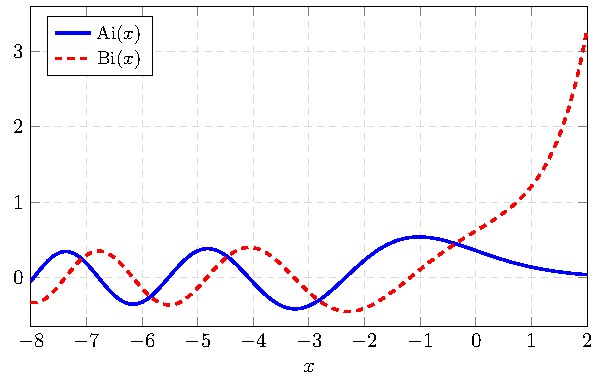
\includegraphics[width=0.81\linewidth]{figs/airy-ai-bi.pdf}
\end{center}
For $x<0$ both oscillate; for $x>0$, $Ai(x)$ decays while $Bi(x)$ grows (formulas
\eqref{eq:airy-neg-asymptotic}--\eqref{eq:airy-pos-asymptotic} at the end of this
chapter).  A condition of decay at $x\to+\infty$ therefore selects $Ai$.
\end{frame}

% ======================================================================
\section{When will the method of Frobenius work?}
% ======================================================================

\begin{frame}[allowframebreaks=1.00]{Classifying the point $x_0$}
\footnotesize

\textbf{The question.} Why are \(zP\) and \(z^2Q\) the right things to test? The answer: they decide
whether the equation looks like an Euler equation near \(x_0\), and Euler equations are solved by
powers.

\textbf{Step 1: look at the equation very close to \(x_0\).} At a regular singular point, \(zP\) and \(z^2Q\)
are analytic, so they have finite values at \(z=0\):
\[
 p_0=\lim_{z\to0}zP(x),\qquad q_0=\lim_{z\to0}z^2Q(x).
\]
Multiply \(y''+Py'+Qy=0\) by \(z^2\) and group the factors as follows:
\[
 z^2y''+(zP)\,zy'+(z^2Q)\,y=0 .
\]
Very close to \(z=0\), replace \(zP\) by \(p_0\) and \(z^2Q\) by \(q_0\). What is left is an Euler equation:
\[
 z^2y''+p_0\,zy'+q_0\,y\approx0.
\]
\textbf{Step 2: the Euler equation is solved by a power.} Try \(y=z^r\): \(y'=rz^{r-1}\), \(y''=r(r-1)z^{r-2}\), so
\[
 z^2y''+p_0zy'+q_0y=\bigl[r(r-1)+p_0r+q_0\bigr]z^r .
\]
This vanishes when \(r\) solves the \emph{indicial equation}
\begin{equation}
 F(r)\equiv r(r-1)+p_0r+q_0=0.
 \label{eq:general-indicial}
\end{equation}
\textbf{Check with Bessel.} \(xP=1\) and \(x^2Q=x^2-m^2\), so \(p_0=1\), \(q_0=-m^2\), and
\(F(r)=r(r-1)+r-m^2=r^2-m^2\). Roots \(r=\pm m\), as found before.
\par\framebreak\par
\textbf{Which roots give a series? The key observation.} Insert the full series
\(y=\sum_ka_kz^{k+r}\). The same computation as in Step~2, with \(r+k\) in place of \(r\), shows that the
term \(a_kz^{k+r}\) produces \(F(r+k)\,a_k\,z^{k+r}\). The remaining parts of \(zP\) and \(z^2Q\) (the terms
\(p_1z,\,q_1z,\dots\)) raise powers, so at the power \(z^{k+r}\) they bring in only earlier coefficients
\(a_0,\dots,a_{k-1}\). So the coefficient of \(z^{k+r}\) reads
\[
 F(r+k)\,a_k+(\text{terms with }a_0,\dots,a_{k-1})=0 .
\]
We can solve for \(a_k\) unless \(F(r+k)=0\), that is, unless \(r+k\) is the \emph{other} root of \(F\).
(Bessel: \(F(\pm m+n)=n(n\pm2m)\), exactly the factors in \eqref{eq:bessel-rec} and
\eqref{eq:bessel-negative-root-rec}.)
\par\framebreak\par
\textbf{Consequences.} Let the roots be \(r_1,r_2\), with \(r_1\) the larger (in real part).
\begin{itemize}
 \item \textbf{Roots not differing by an integer} (complex roots included): starting from either
       root, \(r+k\) never hits the other root. Both roots give Frobenius series.
 \item \textbf{Roots differing by a positive integer \(N\):} starting from \(r_1\), \(r_1+k\) never equals
       \(r_2\), so \(r_1\) always gives a series. Starting from \(r_2\), the step \(k=N\) has \(F(r_2+N)=0\). Then
       the undivided equation decides: it may be consistent (giving a second series) or contradictory (Bessel at \(n=2m\)). If contradictory, the second solution contains
       a logarithm (next frame).
 \item \textbf{Repeated root:} only one series; the second solution contains a logarithm.
\end{itemize}
\textbf{How far do the series converge?} At least up to the nearest other singular point of the
equation, complex ones included (Fuchs' theorem, quoted).
\end{frame}

\begin{frame}[allowframebreaks=1.00]{Where the logarithm in the second solution comes from}
\footnotesize

\textbf{The short answer.} A logarithm appears when building the second solution requires
integrating \(1/x\), since \(\int dx/x=\ln x\).

\textbf{The simplest example:} \(x^2y''+xy'=0\) on \(x>0\).
\begin{itemize}
  \item Try \(y=x^r\): \(r(r-1)+r=r^2=0\). A repeated root \(r=0\), giving only \(y_1=x^0=1\).
  \item Solve exactly instead. Divide by \(x\): \(xy''+y'=0\). The left side is \((xy')'\) by the product
        rule. So \((xy')'=0\), and integrating twice:
        \[
         xy'=C_1,\qquad y'=\frac{C_1}{x},\qquad
         y=C_0+C_1\ln x.
        \]
\end{itemize}
The second solution is \(\ln x\), not another power of \(x\).
\par\framebreak\par
\textbf{Why every repeated root does this.}
\begin{itemize}
  \item \emph{The double root.} \(F(r)=r^2+(p_0-1)r+q_0\). The two roots add up to \(-(p_0-1)=1-p_0\). For a
        double root \(r\), this means \(2r=1-p_0\), that is, \(p_0+2r=1\).
  \item \emph{The second solution.} Later in this chapter (reduction of order) we build a second
        solution from a known one, \(v\), as \(y_2=v\int\frac{e^{-\int P}}{v^2}\).
  \item \emph{Near \(z=0\):} \(v\approx z^r\), and \(P\approx p_0/z\), so \(\int P\approx p_0\ln z\) and
        \(e^{-\int P}\approx z^{-p_0}\). Hence
        \[
         \frac{e^{-\int P}}{v^2}\approx\frac{z^{-p_0}}{z^{2r}}=z^{-(p_0+2r)}=z^{-1},
        \]
        whose integral is \(\ln z\). So \(y_2\approx v\ln z\). (In the example, \(p_0=1\), \(r=0\), \(v=1\).)
\end{itemize}
\textbf{Roots differing by an integer \(N\).} The same computation with \(v\approx z^{r_1}\) gives an integrand
\(z^{-N-1}(1+c_1z+c_2z^2+\cdots)\). Its term \(c_Nz^{-1}\) integrates to \(c_N\ln z\). So a logarithm appears
unless \(c_N=0\), which is the ``consistent'' case of the previous frame.
\end{frame}



% ======================================================================
\section{Second solutions}
% ======================================================================

\begin{frame}[allowframebreaks=1.00]{Reduction of order: building the second solution}
\footnotesize

\textbf{Goal.} Given one solution \(v\) of \(u''+P(x)u'+Q(x)u=0\) (nonzero on the interval of interest),
find a second, independent one. The answer will be
\[
 y_2(x)=v(x)\int^x\frac{e^{-\int^sP}}{v(s)^2}\,ds
 \qquad\text{(precise form: \eqref{eq:reduction}).}
\]
\textbf{Why ``reduction of order''.} Look for the second solution in the form \(y=v\,w\). Then
\(y'=v'w+vw'\) and \(y''=v''w+2v'w'+vw''\). Substituting and grouping the terms that contain \(w\) itself:
\[
 w\,\underbrace{(v''+Pv'+Qv)}_{=0\ (v\text{ is a solution})}+\;v\,w''+(2v'+Pv)\,w'=0 .
\]
What remains involves only \(w'\) and \(w''\): a \emph{first-order} equation for \(w'\). We solve it below in
a neat way, through the Wronskian.
\par\framebreak\par
\textbf{Step 1: an equation for the Wronskian.} We want to get rid of \(Q\). Let \(y\) be any solution.
Multiply \(y''+Py'+Qy=0\) by \(v\), multiply \(v''+Pv'+Qv=0\) by \(y\), and subtract. The \(Q\) terms (\(Qvy\)
in both) cancel:
\[
  vy''-yv''+P(vy'-yv')=0.
\]
Define the \emph{Wronskian} \(W[v,y]=vy'-v'y\). By the product rule,
\(W'=(v'y'+vy'')-(v''y+v'y')=vy''-v''y\). So the display says exactly
\begin{equation}
  W'+PW=0.
  \label{eq:abel-w}
\end{equation}
\textbf{Picture.} \(W\) is the determinant of the matrix
\(\bigl(\begin{smallmatrix}v&y\\v'&y'\end{smallmatrix}\bigr)\), whose columns are the (value, slope) pairs of the two
solutions. If \(y=cv\), the columns are parallel and \(W=0\). So \(W\ne0\) means \(y\) is genuinely different
from \(v\).

\textbf{Step 2: solve for \(W\).} Separate variables in \eqref{eq:abel-w}: \(dW/W=-P\,dx\), so
\(\ln W=-\int P\,dx+\text{const}\). Integrating from a reference point \(x_*\),
\begin{equation}
  W[v,y](x)=C_1
  \exp\left(-\int_{x_*}^{x}P(t)\,dt\right).
  \label{eq:abel-identity}
\end{equation}
This is \emph{Abel's identity}. Note that we found \(W\) without knowing \(y\).
\par\framebreak\par
\textbf{Step 3: recover \(y\) from \(W\).} The quotient rule gives
\((y/v)'=(vy'-yv')/v^2=W/v^2\). Insert \eqref{eq:abel-identity}:
\[
  \left(\frac{y}{v}\right)'
    =\frac{W[v,y]}{v^2}
    =C_1\,\frac{\exp\left(-\int_{x_*}^{x}P(t)\,dt\right)}{v^2(x)}.
\]
Integrate from \(x_*\) to \(x\), then multiply by \(v\). The integration constant \(C_0\) would only add
\(C_0v\), a multiple of the solution we already have, so take \(C_0=0\); and take \(C_1=1\):
\begin{equation}
 y_2(x)=v(x)\int_{x_*}^x
 \frac{\exp\left(-\int_{x_*}^sP(t)\,dt\right)}{v^2(s)}\,ds.
 \label{eq:reduction}
\end{equation}
\textbf{Independence.} By construction \(W[v,y_2]=\exp\bigl(-\int_{x_*}^{x}P\,dt\bigr)\), an exponential,
which is never zero. So \(y_2\) is not a multiple of \(v\).
\end{frame}

\begin{frame}{Reduction-of-order example: harmonic oscillator}
\footnotesize

For $y''+y=0$, take the known solution $v(x)=\cos x$. Here $P(x)=0$.
Work on $(-\pi/2,\pi/2)$, where $v\ne0$, and choose $x_*=0$.
The exponential in \eqref{eq:reduction} is $\exp(-\int_0^s0\,dt)=1$, so
\[
\begin{aligned}
 y_2(x)&=\cos x\int_0^x\frac{ds}{\cos^2s}
       =\cos x\int_0^x\sec^2s\,ds\\
       &=\cos x[\tan s]_0^x
        =\cos x\tan x=\sin x.
\end{aligned}
\]
The independence check uses the derivatives of sine and cosine:
\[
 W[\cos x,\sin x]
 =\cos x\cos x-(-\sin x)\sin x=\cos^2x+\sin^2x=1,
\]
the value $\exp(-\int_0^x0\,dt)=1$ predicted by Step~3.
Thus reduction of order recovers the familiar second solution.
\end{frame}

\begin{frame}[allowframebreaks=1.00]{Reduction-of-order example: Bessel's second solution}
\footnotesize
\textbf{Goal.} For integer \(m\) the root \(r=-m\) gave no series. Build the missing second solution
with the reduction formula \eqref{eq:reduction}, starting from the known solution \(v=J_m\).

\textbf{Step 1: the exponential factor.} Bessel's equation divided by \(x^2\) has \(P(x)=1/x\). Work on an
interval of \((0,\infty)\) where \(J_m\ne0\), with a reference point \(x_*>0\) in it. Then
\[
 \int_{x_*}^{s}\frac{dt}{t}=\ln\frac{s}{x_*},
 \qquad
 \exp\Bigl(-\int_{x_*}^{s}\frac{dt}{t}\Bigr)=e^{-\ln(s/x_*)}=\frac{x_*}{s}.
\]
\textbf{Step 2: the second solution.} Insert this and \(v=J_m\) into \eqref{eq:reduction}:
\(y_2=J_m(x)\int_{x_*}^x\frac{x_*/s}{J_m(s)^2}\,ds\). The constant factor \(x_*\) does not matter (any multiple
of a solution is a solution), so drop it:
\begin{equation}
  \widetilde Y_m(x)=J_m(x)
  \int_{x_*}^{x}\frac{ds}{s\,J_m^2(s)}.
  \label{eq:Ytilde}
\end{equation}
\textbf{Step 3: its Wronskian.} \eqref{eq:reduction} has \(W=e^{-\int P}=x_*/x\); dropping the factor \(x_*\)
divides this by \(x_*\):
\[
 W[J_m,\widetilde Y_m]=\frac1x\neq0 .
\]
\par\framebreak\par
\textbf{Step 4: the standard normalization.} The function used everywhere, \(Y_m\) (full definition in
Chapter~5), is scaled so that
\[
 W[J_m,Y_m]=\frac{2}{\pi x}.
\]
\textbf{Why this number?} It makes \(Y_m\) look like \(J_m\) shifted by a quarter period at large \(x\), the way
\(\sin\) sits next to \(\cos\). Indeed, suppose \(J_m\approx A\cos\theta\) and \(Y_m\approx A\sin\theta\), with
\(A=\sqrt{2/(\pi x)}\) and \(\theta=x-m\pi/2-\pi/4\), so \(\theta'=1\). Ignoring the slow change of \(A\),
\[
 W=J_mY_m'-J_m'Y_m\approx A\cos\theta\cdot A\cos\theta-(-A\sin\theta)\cdot A\sin\theta ,
\]
which is \(A^2(\cos^2\theta+\sin^2\theta)=A^2=\frac{2}{\pi x}\).
\textbf{Step 5: relate \(Y_m\) to \(\widetilde Y_m\).} \(J_m\) and \(\widetilde Y_m\) are two independent solutions, so
every solution is a combination of them: \(Y_m=\alpha\widetilde Y_m+CJ_m\). The Wronskian is linear in its
second slot and \(W[J_m,J_m]=0\), so
\[
 W[J_m,Y_m]=\alpha\,W[J_m,\widetilde Y_m]+C\,W[J_m,J_m]=\frac{\alpha}{x}.
\]
Setting this equal to \(\frac2{\pi x}\) gives \(\alpha=\frac2\pi\):
\begin{equation}
 Y_m(x)=\frac2\pi\widetilde Y_m(x)+C J_m(x).
 \label{eq:Ym}
\end{equation}
The Wronskian fixes the scale \(\frac2\pi\) but not \(C\). (Changing \(x_*\) also changes only \(C\).)
\end{frame}

\begin{frame}[allowframebreaks=1.00]{Near the origin, $Y_m$ blows up}
\footnotesize
\textbf{Goal.} Show that \(Y_m\) is infinite at \(x=0\). This is why a drum, whose displacement is finite at
the center, uses only \(J_m\).

\textbf{Case \(m\ge1\).}
\begin{itemize}
  \item \emph{The integrand.} Near \(0\), \(J_m(s)\approx\frac{s^m}{2^m\,m!}\) (first term of \eqref{eq:Jm}). So
        \[
          s\,J_m^2(s)\approx\frac{s^{2m+1}}{2^{2m}(m!)^2},\qquad
          \frac{1}{sJ_m^2(s)}\approx2^{2m}(m!)^2\,s^{-2m-1}.
        \]
  \item \emph{The integral.} \(\int s^{-2m-1}ds=\frac{s^{-2m}}{-2m}\). The lower limit \(x_*\) only adds a
        constant, so for small \(x\)
        \[
         \int_{x_*}^{x}\frac{ds}{sJ_m^2(s)}\approx-\frac{2^{2m}(m!)^2}{2m}\,x^{-2m}+\text{const}.
        \]
  \item \emph{Multiply by \(J_m(x)\approx\frac{x^m}{2^m\,m!}\).} Using \(\frac{m!}{m}=(m-1)!\):
        \[
         \widetilde Y_m(x)\approx-\frac{2^{2m}(m!)^2}{2m}\,x^{-2m}\cdot\frac{x^m}{2^m\,m!}
         =-\frac{2^{m}\,m!}{2m}\,x^{-m}
         =-2^{m-1}(m-1)!\;x^{-m},
        \]
        which tends to \(-\infty\) as \(x\to0^+\).
\end{itemize}
\par\framebreak\par
\textbf{Case \(m=0\).} \(J_0(s)=1-\frac{s^2}{4}+\cdots\), so \(J_0^2\approx1-\frac{s^2}2\) and
\(\frac{1}{sJ_0^2(s)}\approx\frac1s\bigl(1+\frac{s^2}{2}\bigr)=\frac1s+\frac s2\). Integrating,
\(\int_{x_*}^x\approx\ln x+\text{const}\). Multiplying by \(J_0(x)\approx1\):
\(\widetilde Y_0(x)\approx\ln x\to-\infty\).

\textbf{For \(Y_m\) itself.} By \eqref{eq:Ym}, \(Y_m=\frac2\pi\widetilde Y_m+CJ_m\), and \(CJ_m\) stays bounded. So \(Y_m\)
blows up the same way. (Chapter~5 gives the exact constants.)

\textbf{The hidden logarithm.} For \(m\ge1\) a logarithm is present too, just weaker than \(x^{-m}\). The
expansion of \(1/(sJ_m^2)\) also contains a \(1/s\) term; for example, with
\(J_1(s)=\frac s2\bigl(1-\frac{s^2}{8}+\cdots\bigr)\),
\[
 \frac{1}{sJ_1^2(s)}=\frac{4}{s^3}\Bigl(1-\frac{s^2}{8}+\cdots\Bigr)^{-2}
 =\frac4{s^3}\Bigl(1+\frac{s^2}{4}+\cdots\Bigr)=\frac4{s^3}+\frac1s+\cdots .
\]
The \(1/s\) term integrates to \(\ln x\), so \(\widetilde Y_m\) contains a piece \(J_m(x)\ln x\). This is the
logarithm forced by the failed step \(n=2m\) of the Frobenius recurrence.
\end{frame}

\begin{frame}{The Bessel functions of the second kind $Y_0,\dots,Y_3$}
\footnotesize
\begin{center}
  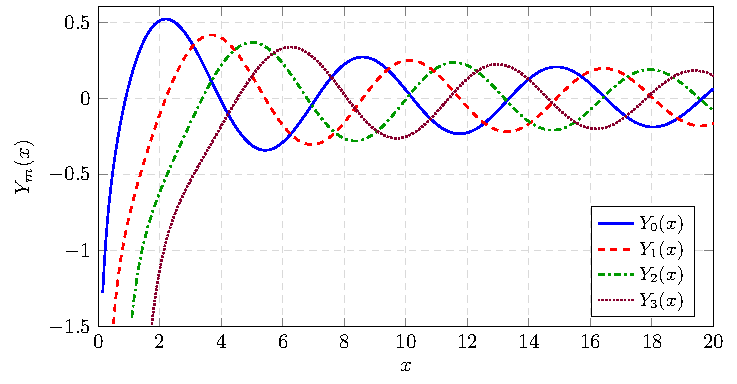
\includegraphics[width=0.86\linewidth]{figs/bessel-Y.pdf}
\end{center}

\medskip
Unlike $J_m$, each $Y_m$ plunges to $-\infty$ as $x\to 0^+$: the second Bessel solution is
singular at the center, so it is excluded for a drum (finite there) but needed on
annular domains.
\end{frame}

% ======================================================================
\section{Airy functions in the complex plane}
% ======================================================================

\begin{frame}[allowframebreaks=1.00]{The Airy integral from a Fourier transform}
\footnotesize
\textbf{Why more than the series.} Applications (for example Chapter~7's quantum particle bouncing
on a floor) need two global facts: which solution decays as \(x\to+\infty\), and where \(Ai\) is zero.
The series hides both. For \(x>0\) every term of \(f_0\) and \(f_1\) is positive, so
\(Ai=Ai(0)f_0+Ai'(0)f_1\) (with \(Ai'(0)<0\)) can decay only through a delicate cancellation. An integral
formula shows these facts directly.

\textbf{Goal.} Find an integral formula for \(Ai\), the solution of \(y''-xy=0\) \eqref{eq:airy} that decays at
\(+\infty\).

\textbf{Why a Fourier transform?} The trouble with \(y''-xy=0\) is the variable coefficient \(x\). Under a
Fourier transform, multiplication by \(x\) turns into a \emph{first} derivative, and \(y''\) turns into
multiplication by \(-t^2\). So the second-order equation becomes a first-order one, which we can
solve at once.
\par\framebreak\par
\textbf{Step 1: the two rules.} Use the convention
\[
 \widehat y(t)=\int_{-\infty}^{\infty}y(x)e^{-itx}\,dx,
 \qquad
 y(x)=\frac1{2\pi}\int_{-\infty}^{\infty}\widehat y(t)e^{itx}\,dt .
\]
\begin{itemize}
  \item \emph{Derivatives become multiplication.} Integrate by parts (the boundary terms vanish when
        \(y\) decays):
        \[
         \widehat{y'}(t)=\int y'e^{-itx}\,dx=\bigl[ye^{-itx}\bigr]-\int y\cdot(-it)e^{-itx}\,dx=it\,\widehat y(t).
        \]
        Applying this twice: \(\widehat{y''}=(it)^2\widehat y=-t^2\,\widehat y\).
  \item \emph{Multiplication by \(x\) becomes a derivative.} Differentiate \(\widehat y\) with respect to \(t\):
        \[
         \frac{d\widehat y}{dt}=\int y(x)\,(-ix)\,e^{-itx}\,dx=-i\,\widehat{(xy)}(t),
         \qquad\text{so}\qquad \widehat{(xy)}=i\,\frac{d\widehat y}{dt}.
        \]
\end{itemize}
\par\framebreak\par
\textbf{Step 2: transform the equation and solve.} By Step~1, \(y''-xy=0\) becomes
\[
 -t^2\,\widehat y-i\,\widehat y\,'=0
 \quad\Longrightarrow\quad
 \widehat y\,'=\frac{-t^2}{i}\,\widehat y=i\,t^2\,\widehat y
 \qquad(\text{using }1/i=-i).
\]
This first-order equation is solved by \(\widehat y(t)=C\,e^{it^3/3}\). (Check: the derivative is
\(C\,e^{it^3/3}\cdot it^2=it^2\,\widehat y\).)

\textbf{Why only one constant?} A second-order equation has two solutions, but only one of them has
a Fourier transform. \(Bi\) grows enormously as \(x\to+\infty\), so its integral \(\widehat y\) does not exist. The
transform automatically picks out the decaying solution. (Making the boundary terms in Step~1
vanish needs a little care, because \(Ai\) decays only slowly as \(x\to-\infty\); we skip this.)
\par\framebreak\par
\textbf{Step 3: transform back.} Insert \(\widehat y=Ce^{it^3/3}\) into the inverse formula:
\[
 y(x)=\frac{C}{2\pi}\int_{-\infty}^{\infty}e^{it^3/3}e^{ixt}\,dt
     =\frac{C}{2\pi}\int_{-\infty}^{\infty}e^{i(t^3/3+xt)}\,dt .
\]
Split the integral at \(t=0\). In the part \(t<0\), substitute \(t\to-t\): the exponent becomes
\(-i(t^3/3+xt)\). So the two halves combine into a cosine, using \(e^{i\phi}+e^{-i\phi}=2\cos\phi\):
\[
 y(x)=\frac{C}{2\pi}\int_0^\infty\Bigl[e^{i(t^3/3+xt)}+e^{-i(t^3/3+xt)}\Bigr]dt
 =\frac{C}{\pi}\int_0^\infty\cos\Bigl(\frac{t^3}{3}+xt\Bigr)dt.
\]
\textbf{Result.} The standard choice is \(C=1\):
\begin{equation}
 Ai(x)=\frac1\pi\int_0^\infty
 \cos\left(\frac{t^3}{3}+xt\right)dt
 \label{eq:airy-integral}
\end{equation}
(an oscillatory integral, understood as the limit of \(\int_0^T\) as \(T\to\infty\)).

\textbf{The constants.} Setting \(x=0\) in \eqref{eq:airy-integral} and evaluating with the gamma
integrals of Chapter~2 reproduces exactly the values \(Ai(0)\) and \(Ai'(0)\) quoted in
\eqref{eq:airy-ic} (we skip this computation). So the integral is the same \(Ai\) as before.
\end{frame}

\begin{frame}[allowframebreaks=1.00]{Large-argument behavior and the zeros of $Ai$}
\footnotesize
\textbf{Goal.} Find how \(Ai\) and \(Bi\) behave for large \(|x|\), and where \(Ai\) is zero. Chapter~7 needs
both: which solution decays as \(x\to+\infty\), and the zeros of \(Ai\).

\textbf{The idea: freeze the coefficient.} In \(y''=xy\), when \(|x|\) is large, the coefficient \(x\) changes
slowly compared with the solution. Over a short stretch near a point \(x_1\), treat it as a constant:
\(y''\approx x_1\,y\).
\begin{itemize}
  \item \(x_1>0\): \(y''=k^2y\) with \(k=\sqrt{x_1}\). Solutions \(e^{\pm kx}\): growth or decay, at the local
        rate \(\sqrt x\).
  \item \(x_1<0\): \(y''=-\kappa^2y\) with \(\kappa=\sqrt{|x_1|}\). Solutions \(\cos\kappa x\), \(\sin\kappa x\):
        oscillation, with the local wave number \(\sqrt{|x|}\).
\end{itemize}
\textbf{Add up the local rates.} Because the rate changes along the way, the total exponent is the
accumulated rate, not rate \(\times\) distance:
\[
 \int_0^x\sqrt s\,ds=\frac23x^{3/2}\quad(x>0),\qquad
 \int_0^q\sqrt s\,ds=\frac23q^{3/2}\quad(x=-q<0).
\]
\textbf{Why the amplitude shrinks on the oscillating side (intuition).} For an oscillator whose
stiffness changes slowly, (amplitude)\(^2\times\)(wave number) stays constant, like a pendulum whose
string is slowly shortened. With wave number \(\sqrt q\), the amplitude goes like \(q^{-1/4}\).
\par\framebreak\par
\textbf{Results} (the constants in front are quoted; they come from a careful analysis of the integral
\eqref{eq:airy-integral}). For \(x\to+\infty\),
\begin{equation}
 Ai(x)\approx\frac{x^{-1/4}}{2\sqrt\pi}\,e^{-\frac23x^{3/2}},
 \qquad
 Bi(x)\approx\frac{x^{-1/4}}{\sqrt\pi}\,e^{+\frac23x^{3/2}}.
 \label{eq:airy-pos-asymptotic}
\end{equation}
For \(x=-q\), \(q\to+\infty\), with the phase \(\chi=\frac23q^{3/2}+\frac\pi4\),
\begin{equation}
 Ai(-q)\approx\frac{q^{-1/4}}{\sqrt\pi}\sin\chi,
 \qquad
 Bi(-q)\approx\frac{q^{-1/4}}{\sqrt\pi}\cos\chi .
 \label{eq:airy-neg-asymptotic}
\end{equation}
The exponents and the phase are the accumulated rates found above. \(Ai\) is the solution that
decays for \(x>0\); \(Bi\) grows.

\textbf{Zeros of \(Ai\).} For \(x>0\), \(Ai\) is positive and decaying. For \(x<0\), by
\eqref{eq:airy-neg-asymptotic}, \(Ai(-q)\approx0\) when \(\sin\chi=0\), that is, \(\chi=p\pi\) with
\(p=1,2,\dots\) (since \(\chi>\frac\pi4\)). Solve for \(q\):
\[
 \frac23q_p^{3/2}+\frac\pi4=p\pi
 \ \Longrightarrow\
 q_p^{3/2}=\frac32\Bigl(p\pi-\frac\pi4\Bigr)=\frac{3\pi(4p-1)}{8}
 \ \Longrightarrow\
 q_p\approx\Bigl[\frac{3\pi(4p-1)}{8}\Bigr]^{2/3}.
\]
This gives \(2.32,\ 4.08,\ 5.52,\dots\); the exact zeros \(x=-q_p\) are at
\(q_p=2.3381,\ 4.0879,\ 5.5206,\dots\), within \(1\%\) already at \(p=1\). (All zeros of \(Ai\) lie on the
negative real axis; quoted.)
\end{frame}


\begin{frame}{Chapter summary}
\scriptsize
\begin{itemize}
  \item A Frobenius expansion has the form
        $y=\sum_{k=0}^{\infty}a_k(x-x_0)^{k+r}$ with $a_0\ne0$.
  \item The lowest-power coefficient gives the indicial equation.  Higher coefficients
        give a recurrence, but every zero recurrence denominator must be checked in the
        original, undivided coefficient equation.
  \item The harmonic oscillator produces the even and odd Taylor chains $\cos x$ and
        $\sin x$.
  \item Bessel's equation has indicial roots $\pm m$.  The regular root gives $J_m$; for
        positive integer $m$, the negative-root branch fails a compatibility equation,
        and the missing solution is $Y_m$.
  \item Airy (ordinary point): Taylor solutions $f_0,f_1$; the decaying $Ai$ has the Fourier
        integral \eqref{eq:airy-integral}; oscillation for $x<0$,
        decay/growth for $x>0$; zeros of $Ai$ at $-q_p$.
  \item Ordinary points have two analytic solutions.  Regular singular points have at
        least one Frobenius solution; an integer root gap may introduce a logarithm or a
        compatibility degeneracy.  Irregular singular points have no general Frobenius
        guarantee.
  \item Reduction of order gives
        \[
          y_2=v\int\frac{e^{-\int P}}{v^2}\,dx,
        \]
        and its nonzero Wronskian proves independence
        from $v$.
\end{itemize}
\end{frame}

\end{document}
